\documentclass[12pt,a4paper]{article}
\linespread{1}
\usepackage[utf8x]{inputenc}
\usepackage[margin=1in]{geometry}
\usepackage{amsmath}
\usepackage{amsthm}
\usepackage{amsfonts}
\usepackage{wrapfig,lipsum,booktabs}
\usepackage{ragged2e}
\usepackage{amssymb}
\usepackage[font=footnotesize,labelfont=bf]{caption}
\usepackage{subcaption}
\usepackage[usenames, dvipsnames]{color}
\usepackage{graphicx}
\usepackage{float}
\usepackage{hhline}
\usepackage{tabularx}
\DeclareUnicodeCharacter{8208}{-}

\newtheorem{theorem}{Theorem}

\newcommand{\rojo}{\textcolor{red}}
\newcommand{\azul}{\textcolor{blue}}

\title{Verifying an Implementation of the Shrinking Bullseye Algorithm}
\begin{document}
\maketitle
\section{Test Model}
To verify that my implementation of the Shrinking Bullseye (SB) is actually working I will use the toy model of a density-dependent SEIR model with normal error and one unknown parameter $\beta$ and the other parameters $\alpha = \gamma = .3$.  The forward model is then given by the differential equation:
\begin{equation}
\vec{f}'(\beta) =
\left[
\begin{array}{c}
- \beta S I\\
\beta S I - .3 E\\
.3 E - .3 I\\
.3 I\\
\end{array}
\right]
\end{equation}
Which I numerically integrate to time $t =3$ (using the SciPy Integrate function `odeint' with 1000 timesteps) to evaluate $\vec{f}(\beta)$.  I create 10 synthetic data points $\vec{d}_i$ where
\[
\vec{d}_i = \vec{f}(\beta^*) + \vec{\epsilon_i}
\]
Where the true parameter value $\beta^* \sim \text{Unif}(0,1.5)$ and the observation error $\vec{\epsilon_i} \sim \text{MVN} \left( (0,10), I_{4 \times 4} \right)$.  I assume a uniform prior with support $[0,10]$, giving the posterior:
\begin{equation}
p(\beta; \vec{d}) \propto \prod\limits_{i=1}^{10} \text{Exp} \left[\frac{-\Vert \vec{f}(\beta) - \vec{d}_i \Vert^2}{10} \right] \mathbf{1}_{[0,10]}(\beta)
\end{equation}
Where $\mathbf{1}$ denotes an indicator function.

Originally I was estimating all three parameters, but the resulting likelihood was extremely narrow.  I tried replacing the multivariate normal error with a binomial error (so the observation process for a noise parameter $p$ and true parameter vector $\theta^*$ was just $\vec{y}_{\text{obs}} = [\text{Binom}(n = \vec{y}(\theta^*)_i,p) \text{ for } i=1,2,3,4]$), but the likelihood was still pretty narrow for reasonable values of $p$.

\section{Running the Sampler}
\textbf{General Sampler Setting: } For 4 SB chains I used a sample size of $7*10e4$ with burn-in of $7*10e3$ steps, a burn-in proposal variance of $.1 I_{4 \times 4}$, and a sampling proposal variance of $.01*I_{4 \times 4}$.  The starting point for each chain was randomly chosen from a uniform distribution over $[0,1.5]$; it would probably be better practice to sample the starting point from the prior, however the posterior is relatively narrow and if the starting point was too far away convergence was incredibly slow.

\textbf{Shrinking Bullseye Settings: } I used quadratic local regressions to start, althought I plan to eventually implement a Gaussian Process regression as well.  For a chain $i$ let $S_i$ denote the set of points in parameter space at which I have pre-evaluated the forward model to use for local regression, and $f(S_i)$ denote the model evaluations at those points.  I constructed $S_i$ by sampling 1000 points from the prior and evaluated $f(S_i)$ at each point.  The initial $S_i$ for each chain was the same, however additional refinements were unique to a chain.  I used the time-dependent cross-validation tolerance of $\omega_t = 0.1t^{-0.1}$ and the random refinement probability $\delta_t = 0.01 t^{-0.2}$ (as chosen by Conrad et. al. in Section 4, ``Numerical Experiments'').  The optimization required at each refinement was performed using the SciPy Optimize function `minimize' with a max iteration of 1000 steps and an additional constraint that the proposed refinement point was in the support of the prior.  This may cause some trouble with the requirement of `goodness of S' that is described in the Appendix of Conrad et. al., but I think if I set the total parameter space $\Theta = [0,10]$ then this will not cause any problems and such a choice seems reasonable for this problem.

One thing I changed in the algorithm was the cross-validation error calculation.  Conrad et. al. have this as $\max_j \left( |min(1,\alpha) - min(1,\alpha^{\sim j})| + |min(1,\frac{1}{\alpha}) - min(1,\frac{1}{\alpha^{\sim j}})| \right)$ where $\alpha^{\sim j}$ is the acceptance probability computed ignoring the $j^{\text{th}}$ point.  Whenever the candidate posterior density was $0$ (which happened pretty regularly, the density curve is pretty narrow) the second term would blow up, so in my implementation I use a cross validation error of just $\max_j \left( |min(1,\alpha) - min(1,\alpha^{\sim j})| \right)$.  It's not a hard fix to implement their formula (I can just add a check to see if $\alpha = 0$ before calculating the error and then set all the $min(1,\frac{1}{\alpha}) = 1$ in that case), but it was cleaner to just use mine instead and I don't think it will ruin the ergodicity of the sampler (the adaptations still diminish over time, but the refinements never completely stop), although it may have adverse effects on its convergence properties. 

\section{Reference Sampler}
Following the methodology of Conrad et. al. I also ran a vanilla Metropolis-Hastings (MH) sampler using the same general settings as the Shrinking Bulleseye sampler.  For all 16 pairings of the 4 SB chains and the 4 MH chains, I compared the relative difference between their mean and variance estimates (ie. the norm of the difference in the SB mean or variance estimate and the MH mean/var estimate, divided by the norm of the MH mean/var estimate) as a function of sampler step $t$.

\section{Results}
Fig. 1 shows a histogram of samplers overlaid with the posterior density curve.  The Gelan-Rubin diagnostic (the version described in Gelman BDA3 that does not include the $\frac{\hat{d}+3}{\hat{d}+1}$ factor) of the fours chains was $\hat{R} = 1.00029$ indicating convergence, although this ignores the fact that the chains may have still been adapting during the sampling phase.  When I ran this chain I had not thought to record what time steps the refinements were occurring at.  I have since updated the script to do so, and run a single chain with a burn-in of $7*10e3$ and a sample size of $10e4$; of 170 refinements that occurred during both burn-in and sampling, 142 of those occurred during the burn-in and during sampling refinements occurred on average every 300 steps (although this isn't a great measure of the refining behavior, as refinements tended to occur in close bursts).

Fig. 2 gives the relative mean and variance error between the SB and reference MH sampler.

The run time of the SB sampler was 4652 seconds (77 minutes), while the MH sampler only took 3902 seconds (65 minutes).  This isn't a great representation of the performance abilities of the SB sampler, as my forward model was pretty quick to run and I think my implementation of the SB has some unnecessary overhead that I'm going to try and reduce in further drafts of the script.

\begin{figure}
  \centering
  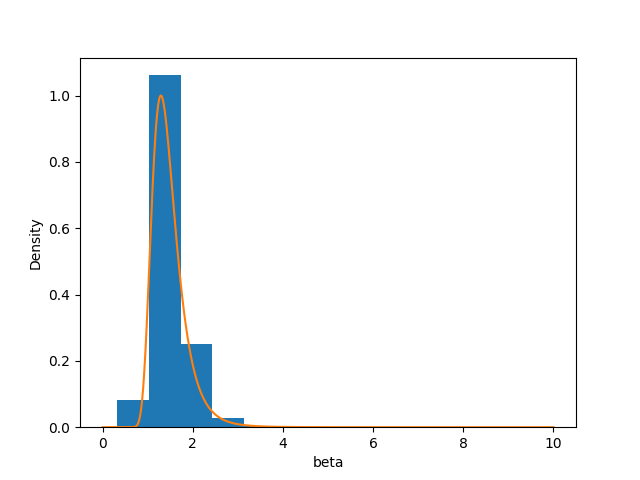
\includegraphics[scale=.5]{./Figs/test_sampler_density.png}
  \caption{Histogram of SB samples (all 4 chains pooled together) against the posterior density curve}
\end{figure}

\begin{figure}
  \begin{tabular}{cc}
    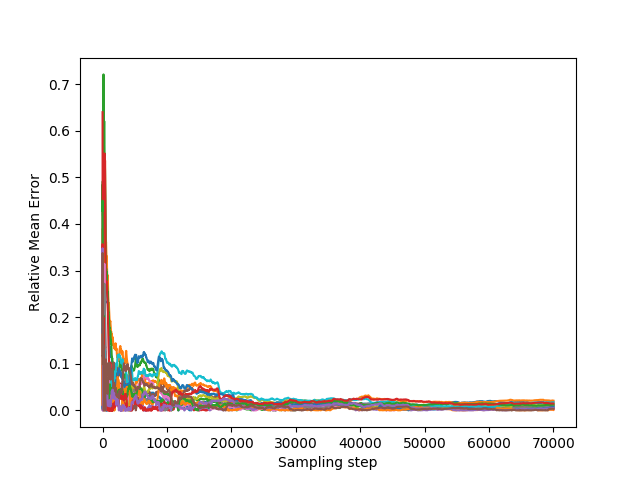
\includegraphics[scale=.5]{./Figs/rel_mean_err.png}  & 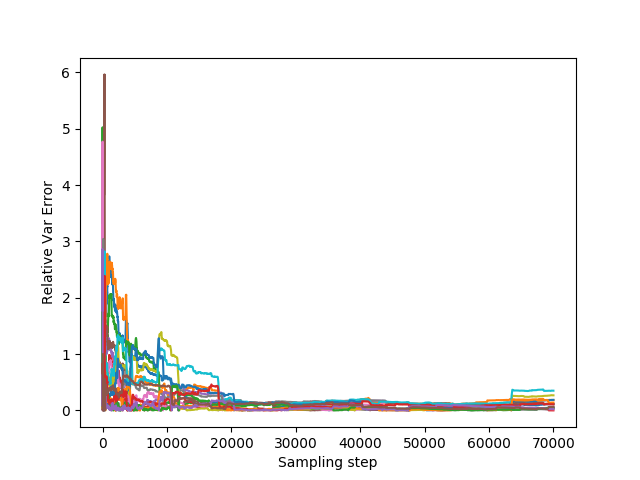
\includegraphics[scale=.5]{./Figs/rel_var_err.png}\\
    (a) & (b)\\
  \end{tabular}
  \caption{(a) The relative mean error of each of the 4 SB chains agains each of the 4 MH chains (so 16 lines in total, since each SB chain was compared to all 4 MH chains), (b) the relative variance error for the same comparisons}
\end{figure}

In general everything seems to be running fine for the SB chains, the samples reflected the posterior density and the chains converged to the same first and second moments as the Metropolis-Hastings chains.  The sampler does work for higher dimensional parameter spaces, although obviously everything gets slowed down.  I can perform this type of verification again for the multi-dimensional case if you think it's important.

\section{Going Forward}
My next steps for this script is to re-write it to reduce overhead and hopefully speed things up.  During the cross-validation stage I'm using a QR row-deletion algorithm from SciPy Linear Algebra, but I want to see if there's something fast I could use.  I'm also going to try this out on a stochastic SIR model; the plan for this is to have the time to each infection and recovery event be exponentially distributed and then use the Gillespie algorithm to simulate this.  I plan to use the average likelihood in the posterior distribution.  The only issue here is that, as it is written by Conrad et. al., the Shrinking Bullseye regresses the forward model on the parameter values, and then evaluating the likelihood function at the regression estimate of the forward model.

Regressing the forward model doesn't really make sense if I'm using an averaged likelihood.  Originally my thought was to regress the average \textit{forward model}, $\bar{f}(\theta)$ on the parameter values, but this doesn't work because we don't have that $L(\bar{f}(\theta)) \neq \bar{L}(f(theta))$ where in both cases the average is taken over stochastic path realizations.  My plan for now is to just tweak the SB to regress the likelihood itelf directly on the parameters, instead of approximating the likelihood through the regressed forward model.  I'm hoping that doing this will preserve Lemmas B.3 and B.8 in Conrad et. al., which (as far as I can tell) is the only part of their ergodicity proof effected by this change.  I haven't verified this fully, however, as the proof is pretty dense.

Eventually I'd like to add either Hamiltonian or Langevin proposal to this sampler, as well as Gaussian process regression, but I think this is lower priority right now.

\end{document}

